\chapter{Flight Testing and Performance Evaluation}\label{ch:performance}

\section{Simulation Results}
Simulation results were captured utilizing the \ac{APM} \ac{SITL} using X-Plane10.  The aircraft model chosen was an open-source flying wing model called the maxi-swift as seen in Figure~\ref{fig:maxi-swift}.

\begin{figure}[!h]
 \centering
  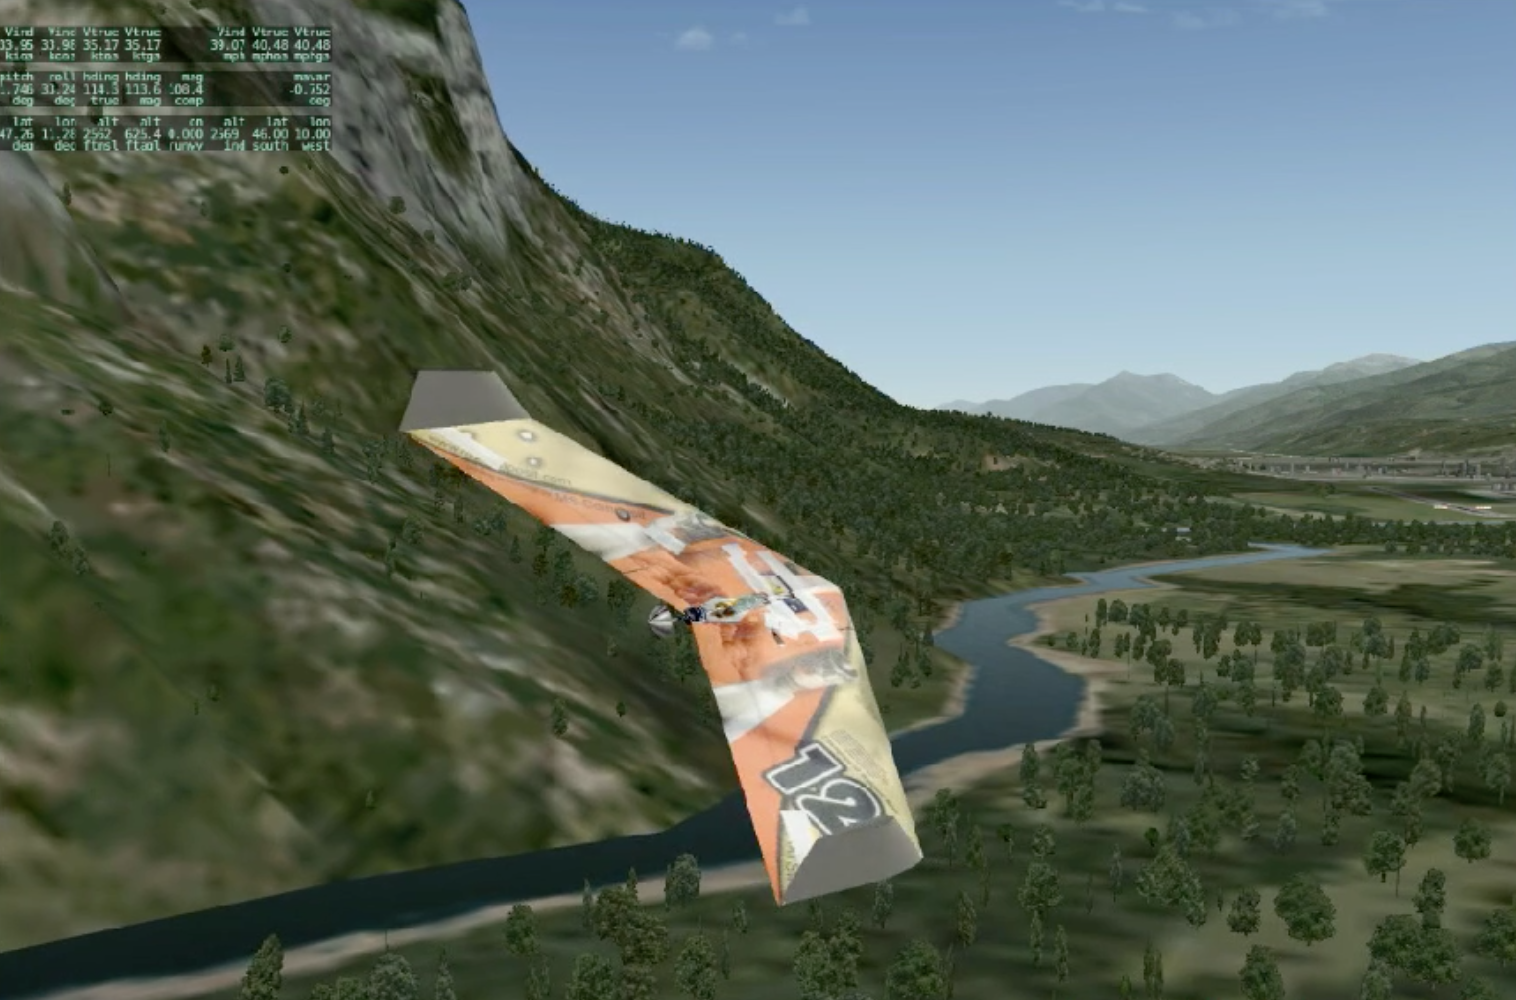
\includegraphics[width=0.75\textwidth]{maxi-swift.png}
  \caption{Maxi-Swift Flying Wing Model used in X-Plane10}
  \label{fig:maxi-swift}
\end{figure}
This plane did not afford proper testing of elevon mixing, but the fidelity in the model provided utilizing X-Plane10 was surprisingly accurate with respect to the FT-Spear aircraft used for actual flight test.  This drastically increased confidence that anything tested in \ac{SITL} would have a high probability of success in actual flight test.


\subsection{Pitch Attitude Performance}

It can be seen in Figure~\ref{fig:pitch_perf} that there exists some steady state error when under \ac{PID} control.  This phenomenon is more pronounced when the desired pitch attitude is negative.  This steady state error is due to the increase in lift caused by the increasing airspeed.  The \ac{PID} controller underperforms in this regime.  However, the adaptive controller is able to compensate for these dynamics fast enough to track the desired attitude with no steady state error.

\begin{figure}[h!]
 \centering
  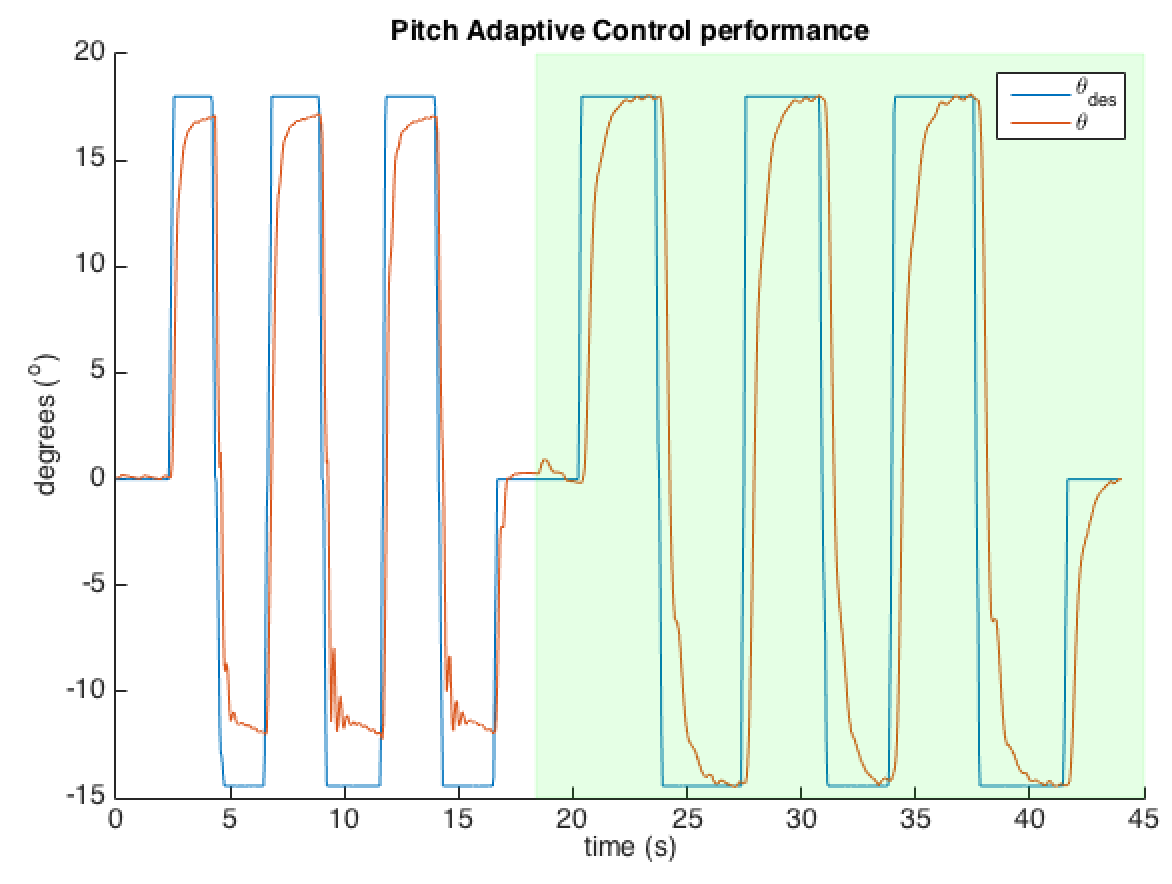
\includegraphics[width=1\textwidth]{pitch_perf.png}
  \caption{PID vs \Lone Adaptive Control Pitch Performance}
  \label{fig:pitch_perf}
\end{figure}

\subsection{Roll Induced Pitch Disturbance}
When rapidly rolling the maxi-swift aircraft in simulation, there was a noticeable coupling in the pitch axis.  The \ac{PID} controller struggles to correct this discrepancy because the time constant of the integral error simply cannot be increased high enough to achieve satisfactory compensation.  As seen in Figure~\ref{fig:pitch_divergence}, the \Lone adaptive controller significantly reduced the pitching disturbance due to rapid rolling.

\begin{figure}[h!]
 \centering
  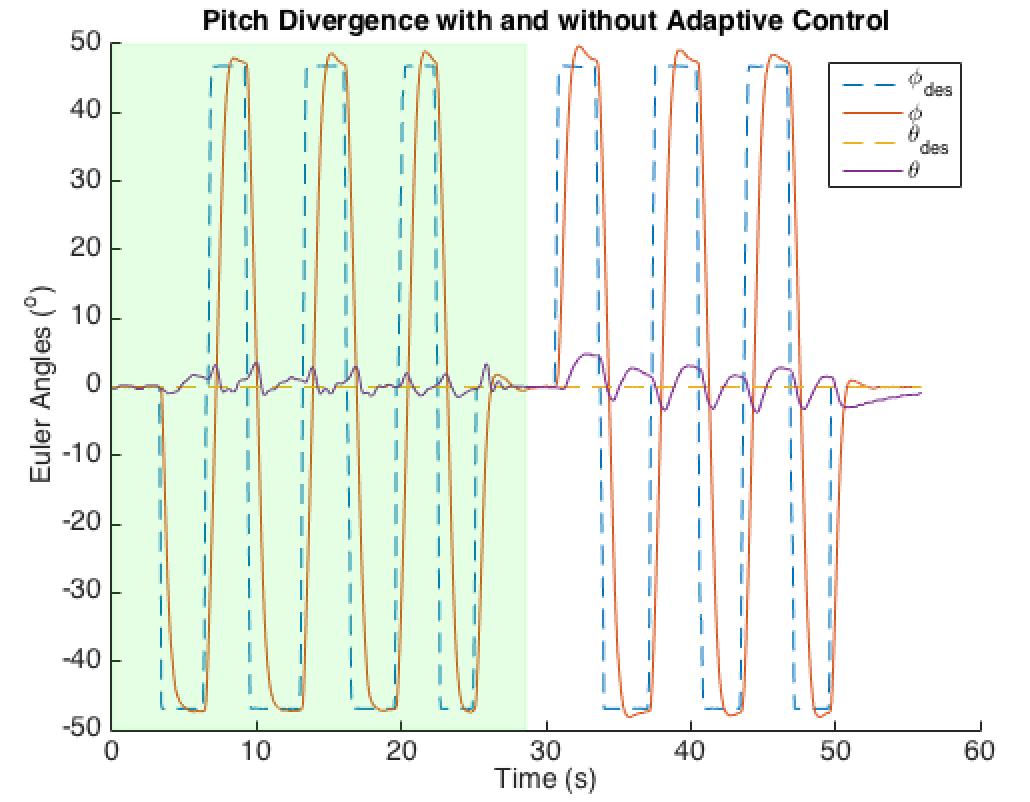
\includegraphics[width=1\textwidth]{pitch_divergence.png}
  \caption{PID vs \Lone Adaptive Control Coupled Pitch Resonse Performance}
  \label{fig:pitch_divergence}
\end{figure}

\subsection{Pitch due to Landing Gear and Flaps}
Lowering the landing gear and flaps entering the landing phase of flight causes un-commanded deviation in pitch.  The F4U Corsair (see Figure~\ref{fig:corsair})in X-Plane10 was used to evaluate the attitude hold retention performance.  This un-modeled aerodynamics can cause the integrator in a \ac{PID} controller to saturate or wind up. 

\begin{figure}[h!]
 \centering
  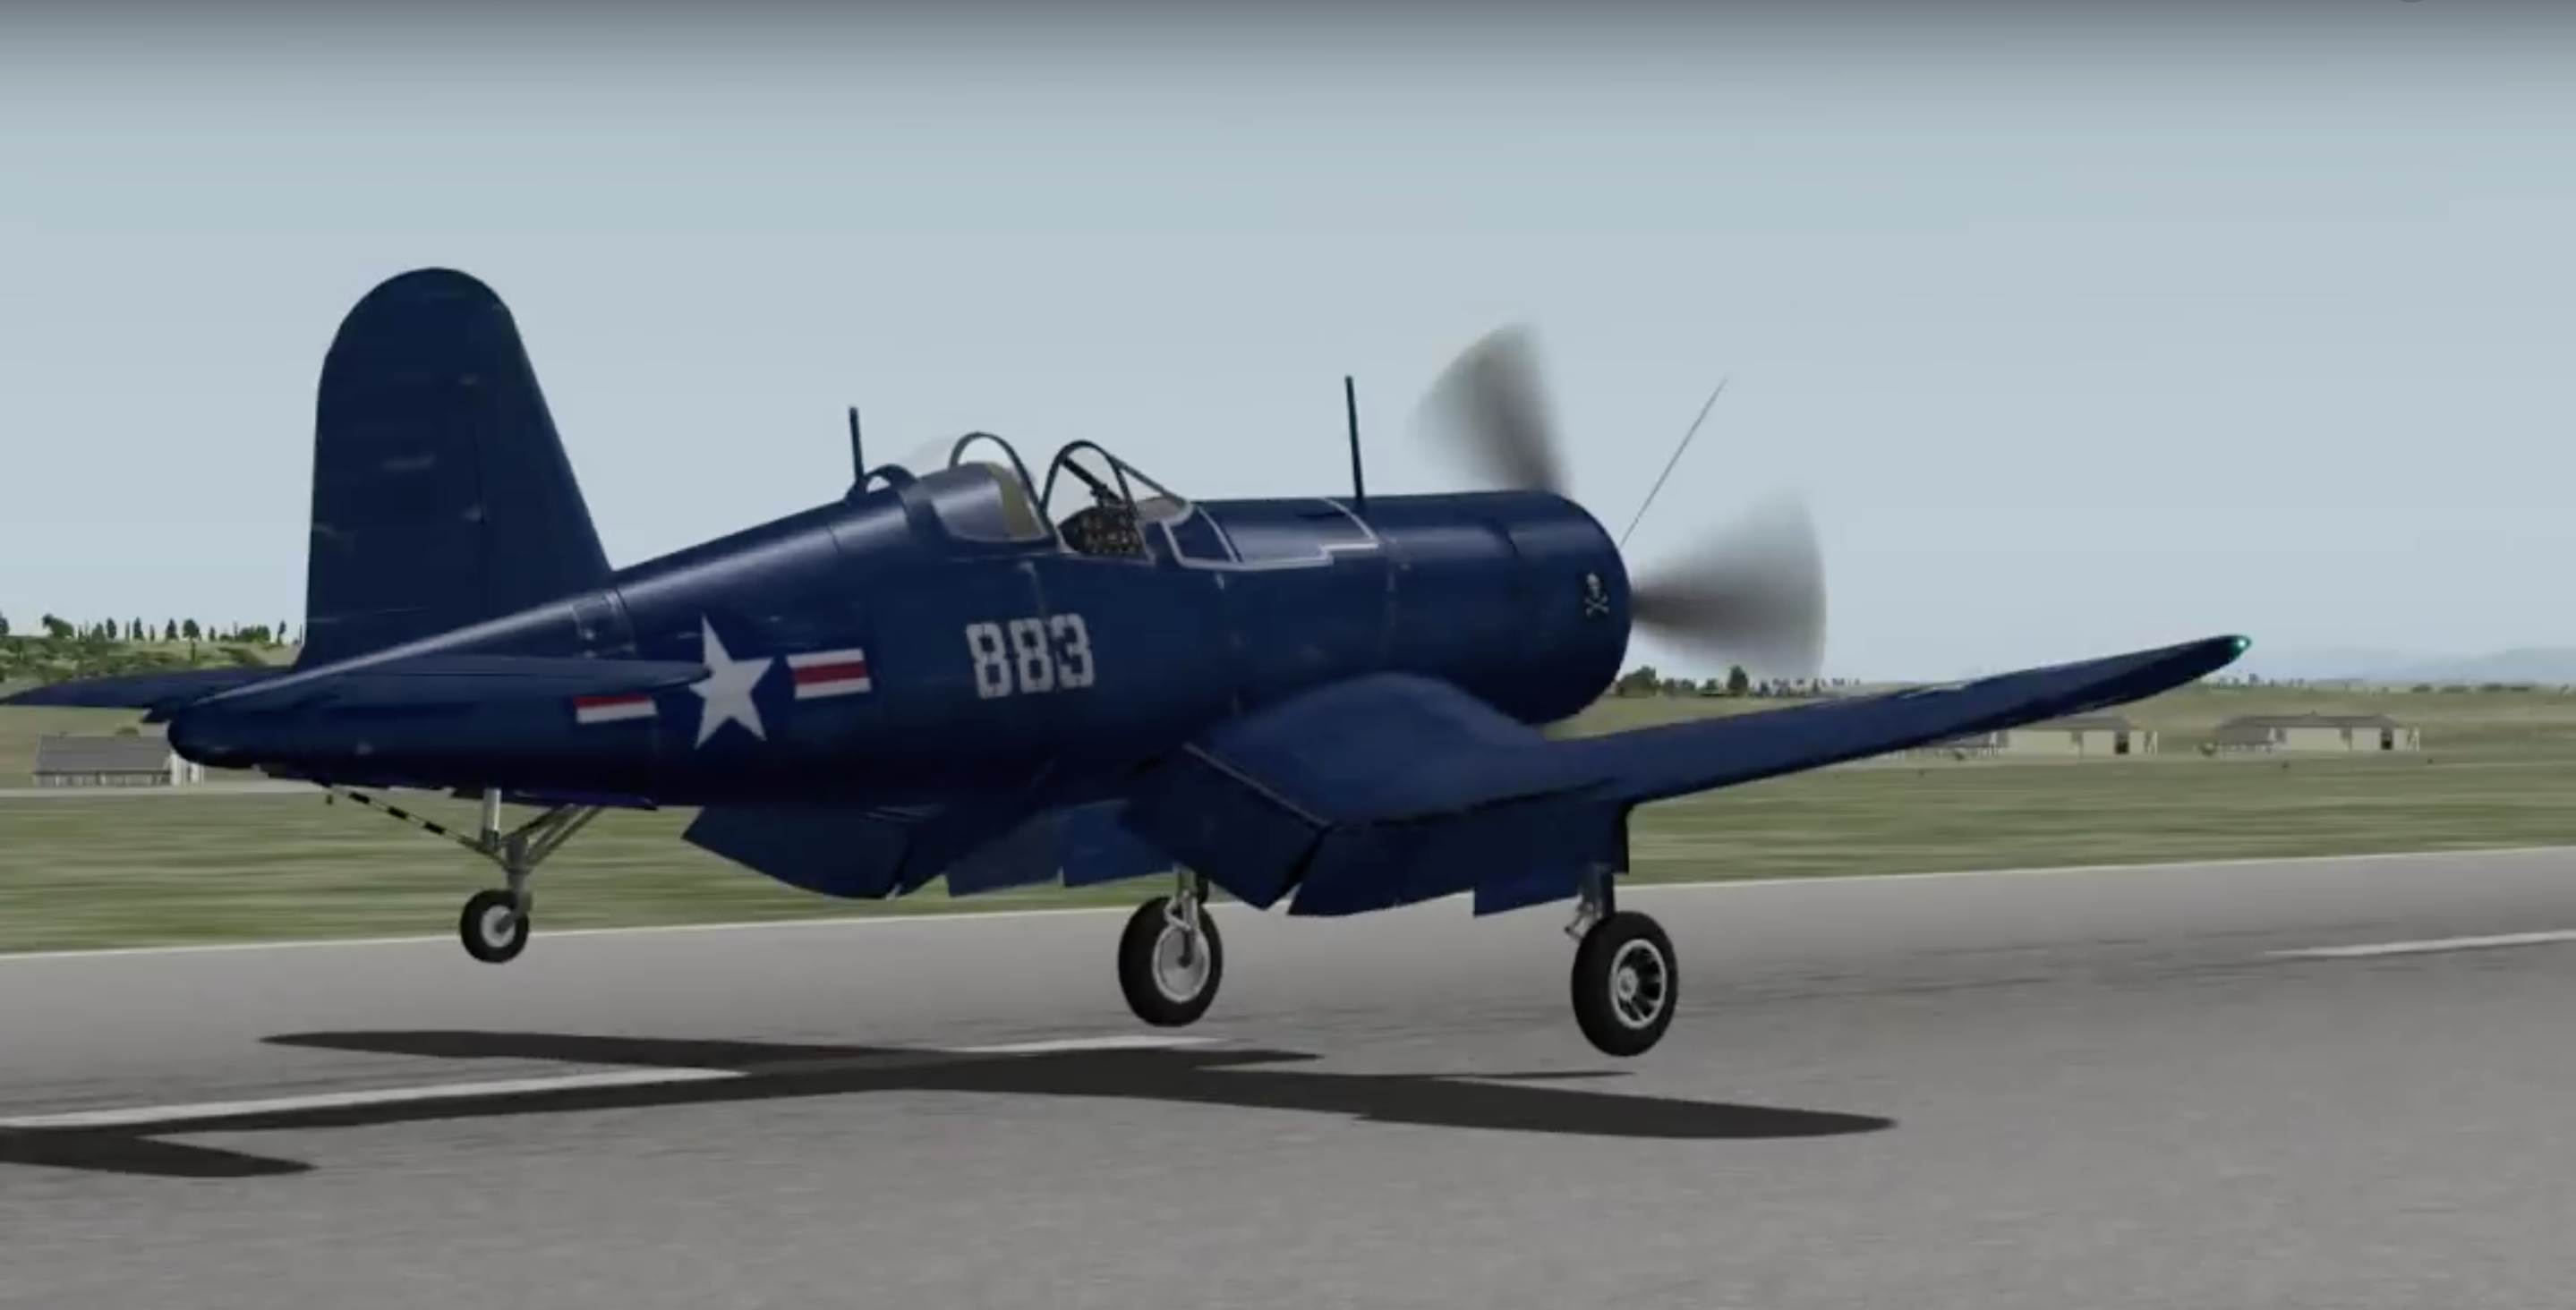
\includegraphics[width=0.85\textwidth]{corsair.png}
  \caption{F4U Corsair model - X-Plane10}
  \label{fig:corsair}
\end{figure}

The \Lone adaptive controller significantly reduces the attitude excursion due to flaps and landing gear.
\begin{figure}[h!]
 \centering
  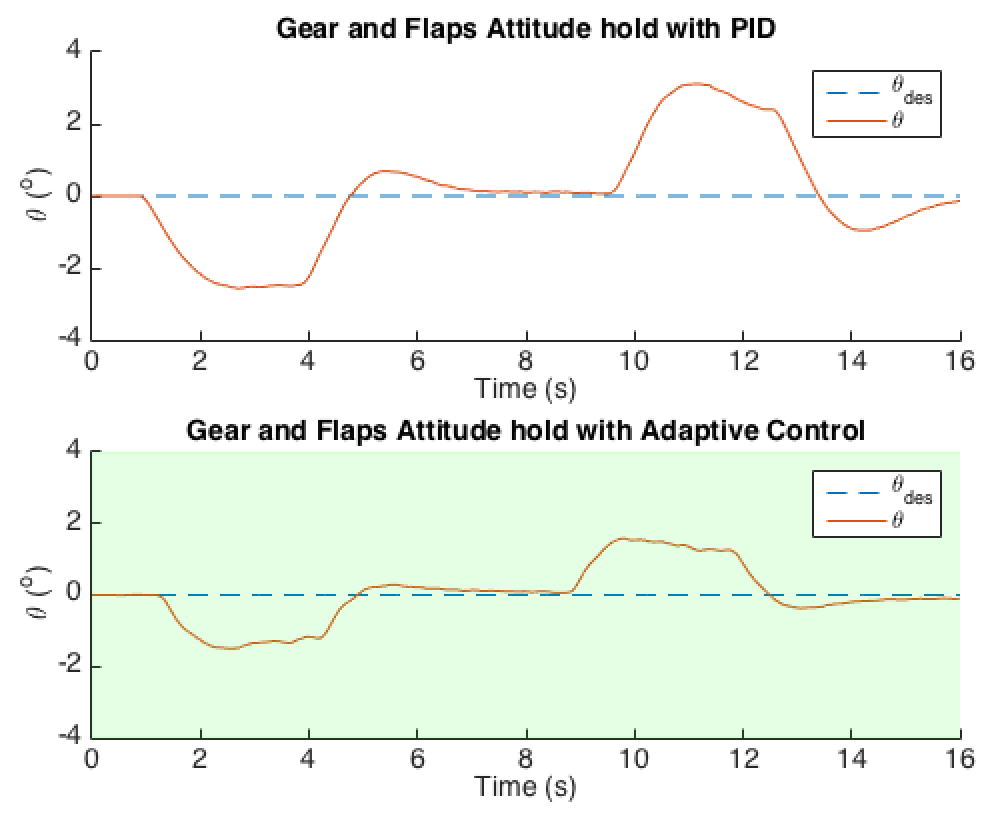
\includegraphics[width=0.85\textwidth]{gear_and_flaps.png}
  \caption{Pitch Attittude Response due to Gear and Flaps}
  \label{fig:gear_and_flaps}
\end{figure}

%---------------------------------------------
\subsection{Roll Performance}
Adaptive control offered little improvement to roll performance with respect to the nominal attitude retention.  The roll axis for multiple aircraft was typically seen to have higher cutoff frequencies with respect to pitch and therefore required higher values for the $D(s)$ cut off frequencies.
\begin{figure}[h!]
 \centering
  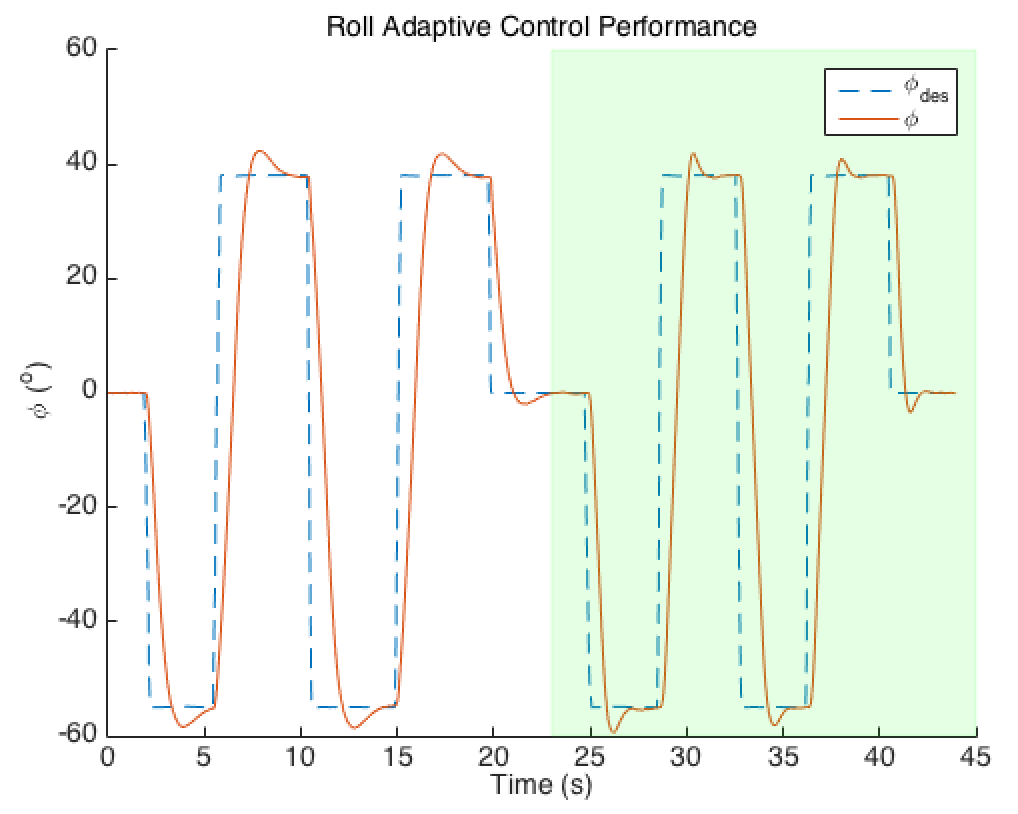
\includegraphics[width=0.85\textwidth]{roll_perf.png}
  \caption{Roll Attittude Performance}
  \label{fig:roll_perf}
\end{figure}

\subsection{Yaw to Roll Coupling}
The roll dynamics are coupled to the yaw dynamics as seen in Equation~\ref{eq:aero_torques}.  In the case of an actuator/servo hardover in the yaw channel, the coupling causes unwanted rolling moments.  Figure~\ref{fig:rudder_failure} compares a left and right yaw servo hard over for both \ac{PID} and the \Lone controller.
\begin{figure}[h!]
 \centering
  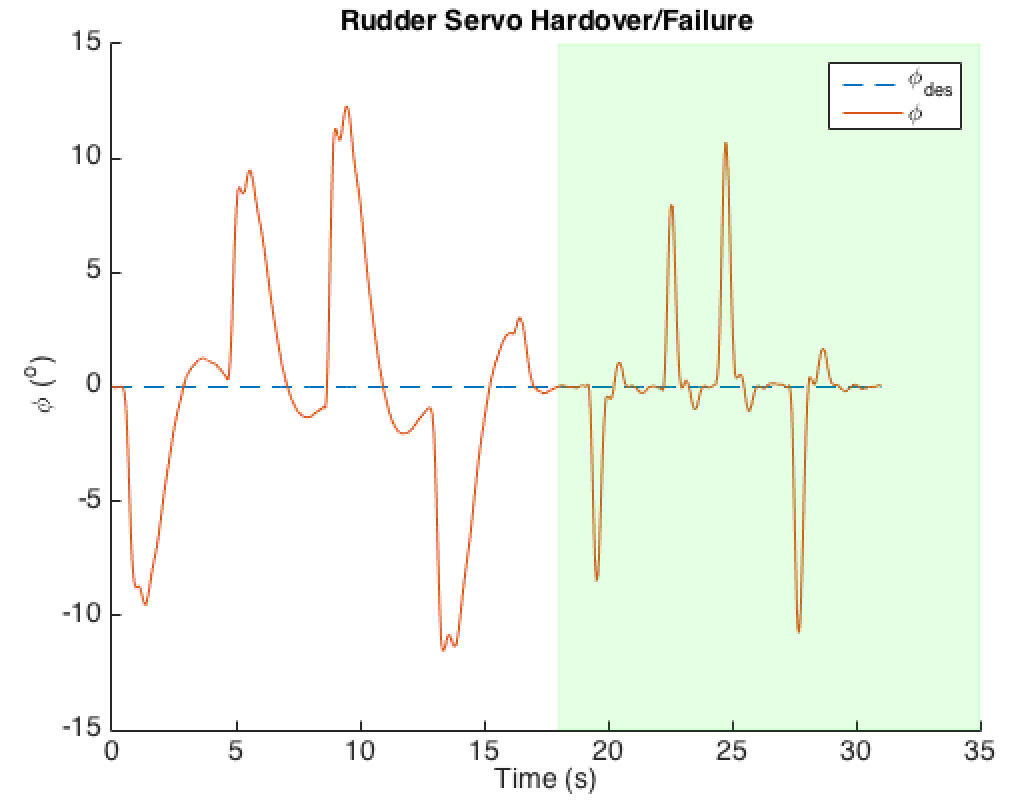
\includegraphics[width=0.85\textwidth]{rudder_failure.png}
  \caption{Roll Response to Rudder Servo Hardover/Failure}
  \label{fig:rudder_failure}
\end{figure}
The adaptive controller significantly outperforms the \ac{PID} controller in maintaining the desired roll.  It could be argued that the \ac{PID} controller's integrator time constant could be re-tuned to be comparable.  It was evident for each of the simulation tests that tuning the \ac{PID} for every scenario would likely have been possible individually to achieve similar performance to the \Lone.  However, the \Lone was not tuned between each of these tests and outperformed \ac{PID} in most, if not all cases.

\subsection{Actuator Miscalibration}
The \Lone adaptive control provided fast learning of airframe actuator miscalibrations.  The autopilot parameter SERVOX\_TRIM was used to offset the ailerons by 15\% of their travel to evaluate how quickly the controller was capable of adapting to the new offset.  This was tested first on the \ac{PID} controller and then on the \Lone as seen in Figure~\ref{fig:trim_learn}.
\begin{figure}[h!]
 \centering
  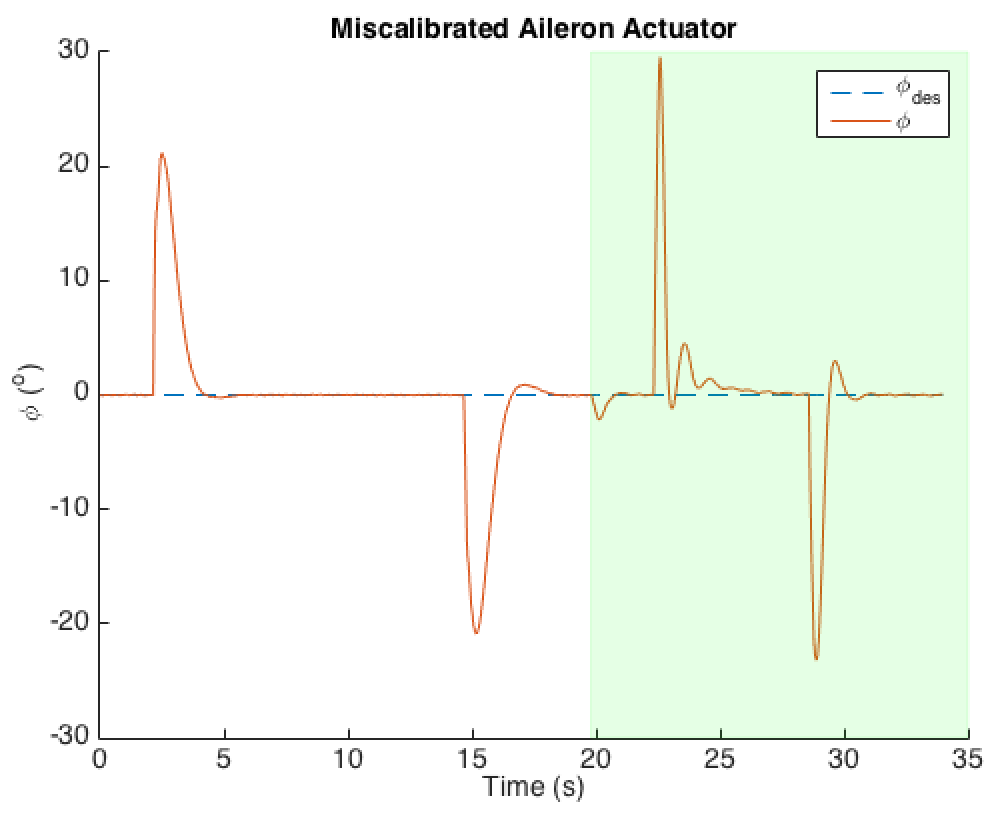
\includegraphics[width=0.65\textwidth]{trim_learn.png}
  \caption{Roll Response to Miscalibrated Aileron Servo}
  \label{fig:trim_learn}
\end{figure}
\begin{figure}[h!]
 \centering
  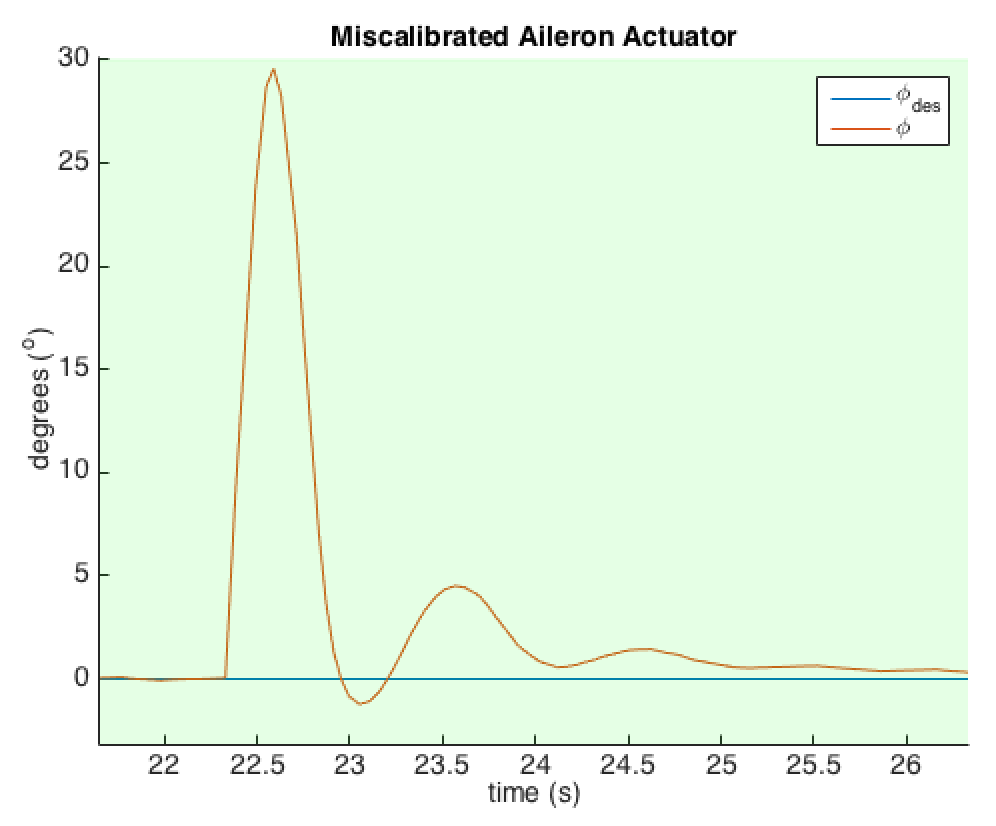
\includegraphics[width=0.65\textwidth]{trim_learn2.png}
  \caption{\Lone Fast Adaptation to Unknown Miscalibration}
  \label{fig:trim_learn2}
\end{figure}

It can be seen in Figure~\ref{fig:trim_learn} and \ref{fig:trim_learn2} that the new trim value achieves the reference command in about 0.5 seconds for the \Lone.  The \Lone is slightly faster than \ac{PID}, but the \Lone exhibits some overshoot.  It is important to note that this rate of learning is perfectly adequate for learning the miscalibrations in flight, but is insufficient for learning on take off.  In the takeoff circumstance, the algorithm saturates the actuator if biases exist between desired and achieved.  Because the aircraft has no dynamic pressure (it is not flying), the desired cannot be achieved.  This causes controller saturation, which cannot be unwound fast enough for take-off (specifically for tail-dragger configuration).  This has to be handled with ad-hoc heuristics very delicately.  One could choose to speed scale the learned parameters to help with learning rate, but it was not chosen for this research because this controller is also utilized in tail-sitter configurations where the zero airspeed would cause the controller to refuse to learn when in \ac{VTOL} mode.

%---------------------------------------------
\section{Flight Test Results}\label{sec:flight_test}
\subsection{General Observations}
The FT Spear aircraft was used in all initial flight tests to prove the algorithm's initial robustness and facilitate testing of various tuning scenarios.  Choosing this aircraft proved to be beneficial because it provided 30 or more minutes of endurance.  The flying wing architecture had a slight forward \ac{CG} when configured with two 2200 \ac{mAh} batteries.  This resulted in the aircraft being anemic in pitch response but still adequate for testing the \Lone algorithm.  Various iterations of the algorithm were tested and compared to the results observed in \ac{SITL} as the development progressed.  

The first observation was that the algorithm, even when poorly tuned, was bounded in response and never approached instability.  The gains found in \ac{SITL} when applied to actual flight test always resulted in stable flight.  As discussed in Section~\ref{sec:tuning}, the first flight tests of gains found in \ac{SITL} either produced low-frequency oscillations or high-frequency oscillations.  Low-frequency oscillations occurred when the \Lone filter cutoff bandwidth was set too low.  High-frequency oscillations occurred when the \Lone filter cutoff bandwidth was set too high.  Tuning the filter to achieve adequate response somewhere between the low and high-frequency oscillations was easily achievable within three to four iterations of setting the filter cutoff frequency.  Finding the optimal filter setting is arguably difficult to see on the low refresh rate telemetry, but achieving similar or better performance than \ac{PID} was easily attained with very minimal effort.

Once the algorithm was well understood and properly implemented in code, flight tests were then conducted on the FT Explorer aircraft.  This aircraft provided more test opportunities because multiple aircraft configurations could be tested with various combinations of flaps and rudder.  

\subsection{Pitch Performance}
As demonstrated in Figure~\ref{fig:pitch_perf}, the simulation results almost identically matched the flight test results for pitch response.  As the aircraft pitches down, the airspeed builds and causes a building steady state error that the integrator time constant struggles to out pace.  This was observed both in simulation and in flight test.  The \Lone adaptive controller's fast adaptation was sufficient to counteract this unmodeled pitching moment.  These results drastically increased the confidence both in the \ac{SITL} fidelity as well as the \Lone adaptive controller.
\begin{figure}[h!]
 \centering
  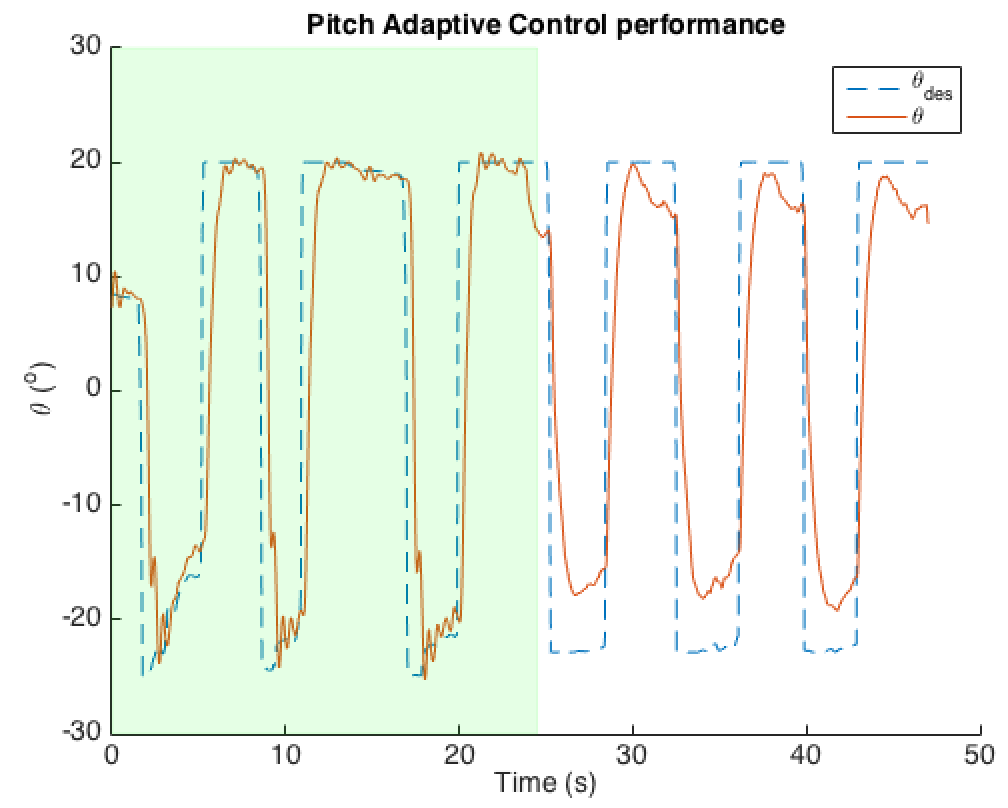
\includegraphics[width=1\textwidth]{pitch_perf_flight_test.png}
  \caption{PID vs \Lone Adaptive Control Pitch Performance}
  \label{fig:pitch_perf_flight_test}
\end{figure}

\subsection{Pitch due to Landing Gear and Flaps}
The \Lone adaptive controller performed well when compensating for the change in aircraft configuration when lowering the flaps.  Figure~\ref{fig:flaps_flight_test} illustrates that the tracking error from lowering and raising the flaps under adaptive control is almost imperceptible.  However, \ac{PID} resulted in a sharp peak both when lowering and raising the flaps.
\begin{figure}[h!]
 \centering
  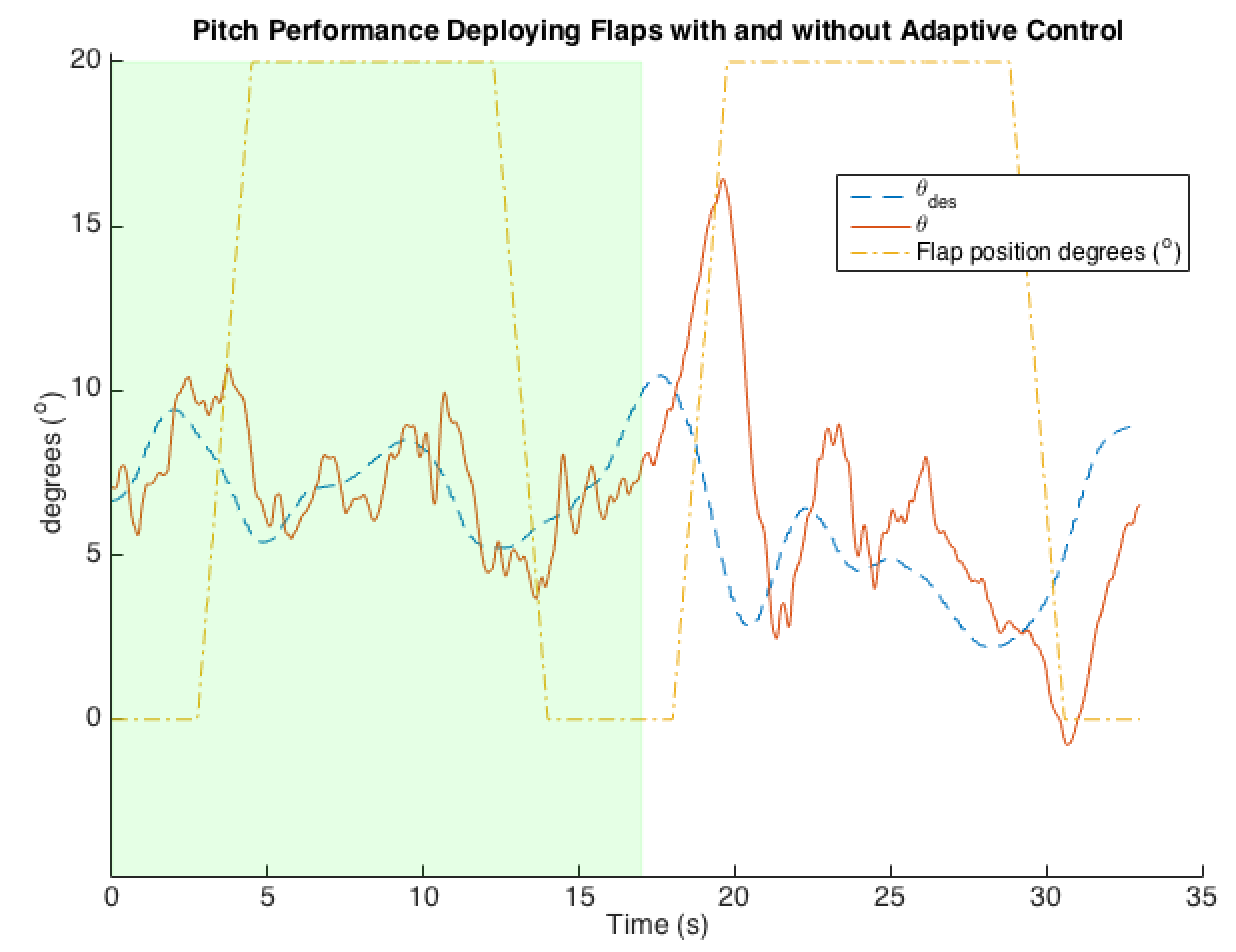
\includegraphics[width=1\textwidth]{flaps_flight_test.png}
  \caption{Pitch Attittude Response due to Gear and Flaps}
  \label{fig:flaps_flight_test}
\end{figure}

\subsection{Roll Induced Pitch Disturbance}
The aircraft max roll angle was set to $\pm$45\degrees to achieve rapid roll while trying to maintain a zero pitch attitude.  This rapid roll maneuver caused significant excursions in pitch when under \ac{PID}.  However, the \Lone controller maintains the pitch attitude within $\pm$3\degrees.  It can be noticed in Figure~\ref{fig:pitch_divergence_flight}, that the adaptive controller oscillates around zero pitch attitude, while the \ac{PID} has more random excursions.  The slight sinusoidal behavior or the \Lone controller is likely due to the cutoff frequency of the filter being slightly too low.  This maneuver may possibly be utilized to fine tune the \Lone's filter cutoff frequency for pitch.
\begin{figure}[h!]
 \centering
  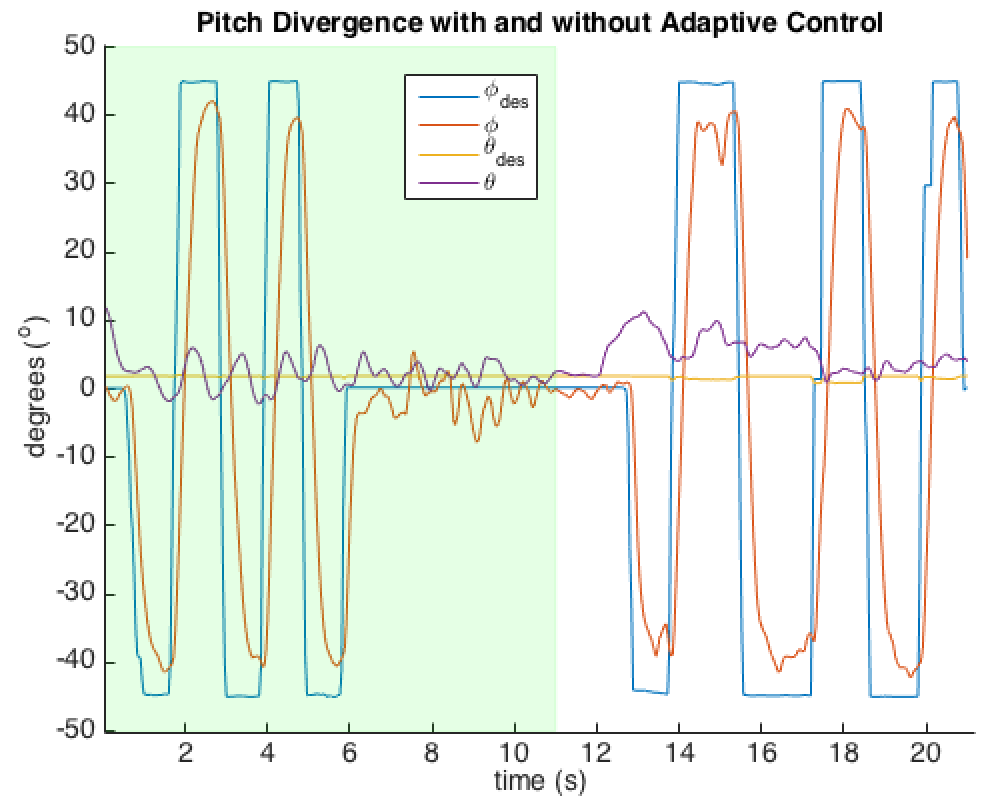
\includegraphics[width=1\textwidth]{pitch_divergence_flight.png}
  \caption{PID vs \Lone Adaptive Control Coupled Pitch Resonse Performance}
  \label{fig:pitch_divergence_flight}
\end{figure}

%---------------------------------------------
\subsection{Roll Performance}
A rectangular flight plan was established to test the nominal flight path stability and roll attitude performance.  Figure~\ref{fig:roll_perf_flight_test} illustrates the \Lone adaptive controller while maintaining the left hand pattern.  The noise in the roll channel was observed in actual flight as turbulence.  The fliter cutoff frequency could be lowered to reduce performance if desired, but these results were not oscillatory which suggested that the filter cutoff frequency was not too high.  These results compare to the noise found on the \ac{PID} channel so the threat of damaging servo by over driving them was not expected.
\begin{figure}[h!]
 \centering
  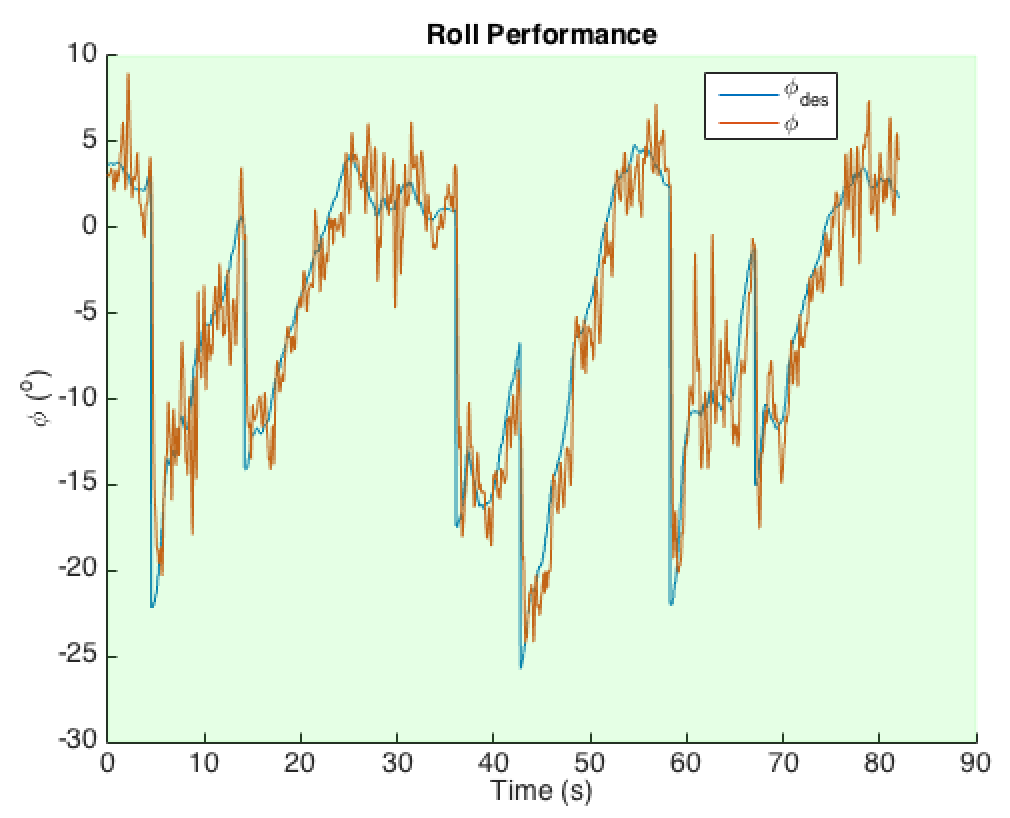
\includegraphics[width=1\textwidth]{roll_perf_flight_test.png}
  \caption{\Lone Adaptive Control Roll Performance}
  \label{fig:roll_perf_flight_test}
\end{figure}

Asymmetric flaps were configured by only allowing one servo to lower the left flap while leaving the right flap stationary.  This failure was designed to test the unmodeled roll response from a very asymmetric mechanical failure.  Unfortunately, the roll and pitch excursions caused by this failure were marginal.  Both \ac{PID} and the \Lone handled this failure with adequate reliability. 


